\documentclass[12pt,a4paper]{article}
\usepackage[utf8]{inputenc}
\usepackage[margin=1in]{geometry}
\usepackage{amsmath}
\usepackage{graphicx}
\usepackage{booktabs}
\usepackage{hyperref}
\usepackage{fancyhdr}
\usepackage{titlesec}
\usepackage{xcolor}
\usepackage{float}
\usepackage{tikz}
\usetikzlibrary{shapes.geometric, arrows, positioning}

% Fix headheight warning
\setlength{\headheight}{14.49998pt}
\addtolength{\topmargin}{-2.49998pt}

% Page headers
\pagestyle{fancy}
\fancyhf{}
\fancyhead[L]{Weather Prediction Machine Learning Project}
\fancyhead[R]{\thepage}
\renewcommand{\headrulewidth}{0.4pt}

% Section formatting
\titleformat{\section}{\large\bfseries\color{blue!70!black}}{\thesection}{1em}{}
\titleformat{\subsection}{\normalsize\bfseries}{\thesubsection}{1em}{}

% Title
\title{\LARGE\textbf{Weather Prediction Machine Learning Project}}
\author{}
\date{}

\begin{document}

\maketitle
\newpage

\section{Introduction}

This project develops machine learning models to classify weather conditions using the Seattle Weather Dataset. The dataset contains daily weather observations with features like precipitation, temperature (max/min), and wind speed. The goal is to classify weather into 5 types: rain, sun, drizzle, snow, and fog. The dataset has approximately 1,460 observations with imbalanced classes.

\subsection{Objectives}

The project aims to test multiple machine learning algorithms for weather classification, handle class imbalance using SMOTEENN technique, optimize models through hyperparameter tuning, compare ensemble methods (Voting and Stacking), and evaluate model performance using multiple metrics.

\section{Methodology}

\subsection{Process Flow}

Figure \ref{fig:process} shows the complete workflow of the weather prediction system.

\begin{figure}[H]
\centering
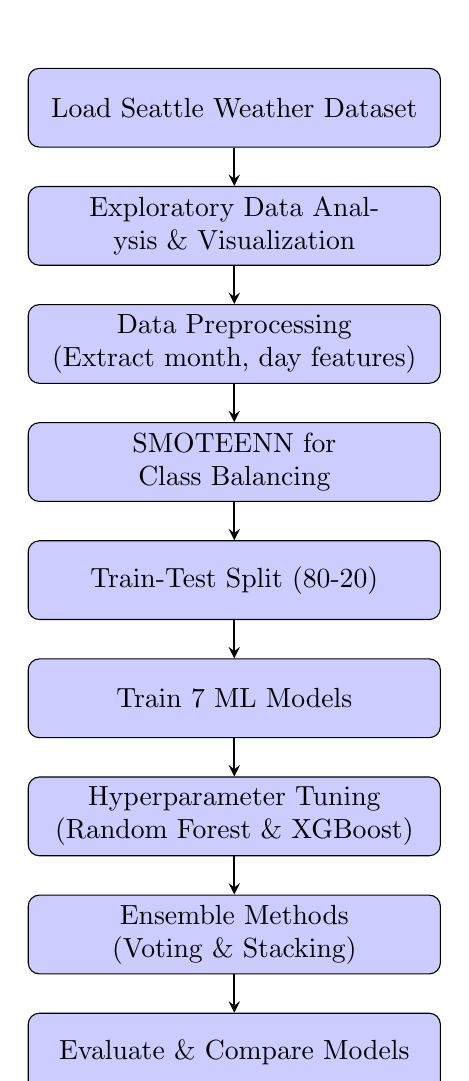
\begin{tikzpicture}[node distance=1.5cm, auto,
    box/.style={rectangle, draw, fill=blue!20, text width=5cm, text centered, rounded corners, minimum height=1cm},
    arrow/.style={thick,->,>=stealth}]
    
    \node[box] (data) {Load Seattle Weather Dataset};
    \node[box, below of=data] (eda) {Exploratory Data Analysis \& Visualization};
    \node[box, below of=eda] (prep) {Data Preprocessing \\ (Extract month, day features)};
    \node[box, below of=prep] (smote) {SMOTEENN for Class Balancing};
    \node[box, below of=smote] (split) {Train-Test Split (80-20)};
    \node[box, below of=split] (train) {Train 7 ML Models};
    \node[box, below of=train] (tune) {Hyperparameter Tuning \\ (Random Forest \& XGBoost)};
    \node[box, below of=tune] (ensemble) {Ensemble Methods \\ (Voting \& Stacking)};
    \node[box, below of=ensemble] (eval) {Evaluate \& Compare Models};
    
    \draw[arrow] (data) -- (eda);
    \draw[arrow] (eda) -- (prep);
    \draw[arrow] (prep) -- (smote);
    \draw[arrow] (smote) -- (split);
    \draw[arrow] (split) -- (train);
    \draw[arrow] (train) -- (tune);
    \draw[arrow] (tune) -- (ensemble);
    \draw[arrow] (ensemble) -- (eval);
\end{tikzpicture}
\caption{Weather Prediction Process Flow}
\label{fig:process}
\end{figure}

\subsection{Algorithms Implemented}

Seven machine learning algorithms were implemented in this project. Logistic Regression serves as a linear classifier for baseline performance. Decision Tree provides a non-linear tree-based model. Support Vector Machine (SVM) finds optimal decision boundaries in the feature space. Random Forest creates an ensemble of decision trees. K-Nearest Neighbors (KNN) uses distance-based classification. AdaBoost implements adaptive boosting ensemble technique. Finally, XGBoost employs gradient boosting with regularization for improved performance.

\subsection{Algorithm Formulations}

\textbf{Logistic Regression:} The probability of class $y=1$ is modeled using the sigmoid function:
$$P(y=1|x) = \frac{1}{1 + e^{-(\beta_0 + \beta_1 x_1 + ... + \beta_n x_n)}}$$

\textbf{Decision Tree:} Split criterion using Gini impurity:
$$Gini = 1 - \sum_{i=1}^{C} p_i^2$$
where $p_i$ is the probability of class $i$ and $C$ is the number of classes.

\textbf{Support Vector Machine (SVM):} The decision function finds the optimal hyperplane:
$$f(x) = sign(w^T x + b)$$
subject to maximizing the margin $\frac{2}{||w||}$.

\textbf{Random Forest:} Ensemble prediction by averaging multiple decision trees:
$$\hat{y} = \frac{1}{T} \sum_{t=1}^{T} h_t(x)$$
where $T$ is the number of trees and $h_t(x)$ is the prediction of tree $t$.

\textbf{K-Nearest Neighbors (KNN):} Classification based on majority vote:
$$\hat{y} = \text{mode}\{y_i : x_i \in N_k(x)\}$$
where $N_k(x)$ represents the $k$ nearest neighbors of $x$.

\textbf{AdaBoost:} Weighted combination of weak learners:
$$F(x) = \sum_{t=1}^{T} \alpha_t h_t(x)$$
where $\alpha_t = \frac{1}{2}\ln\frac{1-\epsilon_t}{\epsilon_t}$ and $\epsilon_t$ is the weighted error.

\textbf{XGBoost:} Gradient boosting objective function:
$$\mathcal{L} = \sum_{i=1}^{n} l(y_i, \hat{y}_i) + \sum_{k=1}^{K} \Omega(f_k)$$
where $l$ is the loss function and $\Omega$ is the regularization term.

\section{Data Analysis}

\subsection{Exploratory Data Analysis}

The dataset contains 1,461 observations with no missing values. Weather type distribution shows significant class imbalance with rain and sun as majority classes.

\begin{figure}[H]
\centering
\includegraphics[width=0.6\textwidth]{weather type distribution.png}
\caption{Weather Type Distribution showing class imbalance}
\label{fig:weather_dist}
\end{figure}

\subsection{Feature Correlation}

Correlation analysis reveals relationships between meteorological features. Temperature features (max and min) show strong positive correlation.

\begin{figure}[H]
\centering
\includegraphics[width=0.6\textwidth]{corr heatmap.png}
\caption{Correlation Heatmap of numerical features}
\label{fig:corr}
\end{figure}

\subsection{Feature Distributions}

Analysis of feature distributions shows precipitation is right-skewed while temperature features are more normally distributed.

\begin{figure}[H]
\centering
\includegraphics[width=0.8\textwidth]{different distributions.png}
\caption{Distribution of weather features}
\label{fig:distributions}
\end{figure}

\section{Data Preprocessing}

\subsection{Feature Engineering}

Date features were extracted to capture temporal patterns in the weather data. Specifically, the month feature captures seasonal variation, while the day feature identifies daily patterns. After extracting these temporal features, the original date column was dropped as it was no longer needed for modeling.

\subsection{Class Imbalance Handling}

SMOTEENN (Synthetic Minority Over-sampling Technique + Edited Nearest Neighbours) was applied to balance the dataset. This technique oversamples minority classes by creating synthetic examples through interpolation, removes noisy samples using nearest neighbors analysis, and ultimately improves model performance on minority classes. The balanced dataset increased from 1,461 to 2,174 samples with more equal representation across all weather types.

\subsection{Train-Test Split}

Data was split into training and testing sets following an 80-20 ratio, with 80\% of the data used for training and 20\% reserved for testing. Labels were encoded numerically using LabelEncoder for model compatibility.

\section{Model Training and Results}

\subsection{Initial Model Performance}

All seven algorithms were trained on the balanced dataset. Table \ref{tab:baseline} shows actual results from the notebook.

\begin{table}[H]
\centering
\caption{Initial Model Performance (Actual Results)}
\label{tab:baseline}
\begin{tabular}{lc}
\toprule
\textbf{Model} & \textbf{Accuracy} \\
\midrule
Logistic Regression & 0.7609 \\
Decision Tree & 0.9218 \\
SVM & 0.7701 \\
Random Forest & 0.9609 \\
KNN & 0.9287 \\
AdaBoost & 0.4736 \\
XGBoost & 0.9609 \\
\bottomrule
\end{tabular}
\end{table}

Random Forest and XGBoost achieved the highest accuracy (96.09\%), followed by KNN (92.87\%) and Decision Tree (92.18\%). Logistic Regression and SVM performed moderately (76-77\%), while AdaBoost showed the poorest performance at 47.36\%.

\subsection{Hyperparameter Tuning}

GridSearchCV was used to optimize Random Forest and XGBoost models. For Random Forest, the parameters tested included n\_estimators with values [100, 200], max\_depth with values [10, 20], and min\_samples\_split with values [2, 5]. The best parameters found were max\_depth of 20, min\_samples\_split of 2, and n\_estimators of 200, achieving a tuned accuracy of 0.9678.

For XGBoost, the hyperparameter search explored n\_estimators [100, 200], max\_depth [5, 7], and learning\_rate [0.1, 0.2]. The optimal configuration was determined to be learning\_rate of 0.2, max\_depth of 7, and n\_estimators of 200, resulting in a tuned accuracy of 0.9632.

Both models showed improved performance after tuning, with Random Forest improving from 96.09\% to 96.78\% and XGBoost improving from 96.09\% to 96.32\%.

\subsection{Ensemble Methods}

Two ensemble approaches were implemented in this project. The Voting Classifier combines tuned Random Forest, KNN, and tuned XGBoost using soft voting (probability-based), achieving 97.70\% accuracy. The Stacking Classifier employs Logistic Regression, Decision Tree, Random Forest, and KNN as base models, with Logistic Regression serving as the meta-model, and achieved 98.39\% accuracy, representing the highest performance among all models tested.

\section{Results}

\subsection{Final Model Comparison}

Table \ref{tab:final} shows the complete performance comparison of all models.

\begin{table}[H]
\centering
\caption{Complete Model Performance Results}
\label{tab:final}
\begin{tabular}{lcccc}
\toprule
\textbf{Model} & \textbf{Accuracy} & \textbf{Precision} & \textbf{Recall} & \textbf{F1-Score} \\
\midrule
Stacking Ensemble & 0.9839 & 0.9843 & 0.9839 & 0.9840 \\
Voting Ensemble & 0.9770 & 0.9776 & 0.9770 & 0.9770 \\
Random Forest (Tuned) & 0.9678 & 0.9691 & 0.9678 & 0.9675 \\
XGBoost (Tuned) & 0.9632 & 0.9645 & 0.9632 & 0.9631 \\
Random Forest & 0.9609 & 0.9632 & 0.9609 & 0.9596 \\
XGBoost & 0.9609 & 0.9617 & 0.9609 & 0.9608 \\
KNN & 0.9287 & 0.9326 & 0.9287 & 0.9275 \\
Decision Tree & 0.9218 & 0.9261 & 0.9218 & 0.9192 \\
SVM & 0.7701 & 0.8087 & 0.7701 & 0.7614 \\
Logistic Regression & 0.7609 & 0.7684 & 0.7609 & 0.7607 \\
AdaBoost & 0.4736 & 0.5475 & 0.4736 & 0.4692 \\
\bottomrule
\end{tabular}
\end{table}

\subsection{Model Comparison Visualization}

Figure \ref{fig:comparison} shows the performance comparison of the top models.

\begin{figure}[H]
\centering
\includegraphics[width=0.8\textwidth]{Model performance comparison.png}
\caption{Performance comparison of best models}
\label{fig:comparison}
\end{figure}



The Stacking Classifier achieved the highest accuracy at 98.39\%, followed by the Voting Ensemble at 97.70\%. Both ensemble methods outperformed individual models, demonstrating the effectiveness of combining multiple algorithms.

\section{Results and Analysis}

Comprehensive evaluation of all implemented approaches reveals that ensemble methods significantly outperformed individual models. The Stacking Classifier achieved the best performance with 98.39\% accuracy, followed by the Voting Ensemble at 97.70\%. These results demonstrate that combining multiple algorithms effectively captures the complex patterns in weather data.

Among individual models, Random Forest and XGBoost (both tuned) showed strong performance with 96.78\% and 96.32\% accuracy respectively. Tree-based models (Random Forest, XGBoost, Decision Tree) generally performed well on the balanced dataset. KNN achieved 92.87\% accuracy, while linear models (Logistic Regression and SVM) showed moderate performance at 76-77\%. AdaBoost struggled significantly with only 47.36\% accuracy, indicating poor suitability for this specific dataset.

\subsection{Key Findings}

The analysis reveals several important findings from this weather prediction project. SMOTEENN successfully balanced the imbalanced dataset, enabling better model performance across all weather classes. Hyperparameter tuning improved Random Forest from 96.09\% to 96.78\% and XGBoost from 96.09\% to 96.32\%. Ensemble methods achieved the best results, with Stacking reaching 98.39\% and Voting achieving 97.70\% accuracy. Tree-based models including Random Forest, XGBoost, and Decision Tree performed well on the balanced dataset. Linear models such as Logistic Regression and SVM showed moderate performance at 76-77\%. AdaBoost showed the poorest performance at 47.36\%, indicating its poor suitability for this specific dataset.

\section{Conclusion}

This project successfully developed machine learning models to predict weather conditions. Seven different algorithms were tested including Logistic Regression, Decision Tree, SVM, Random Forest, KNN, AdaBoost, and XGBoost.

The SMOTEENN technique effectively balanced the imbalanced dataset, allowing models to learn patterns from minority classes. Hyperparameter tuning improved model performance, and ensemble approaches worked better than individual models for this weather classification task.

The Stacking Classifier achieved the highest accuracy at 98.39\%, followed by the Voting Ensemble at 97.70\%. This demonstrates that combining multiple models captures complex weather patterns more effectively than individual algorithms. The balanced dataset from SMOTEENN enabled better performance on minority weather classes.

\end{document}
